% Created 2024-09-23 Mon 13:35
% Intended LaTeX compiler: pdflatex
%%% TeX-command-extra-options: "-shell-escape"

\documentclass{iacrtrans}
\usepackage[utf8]{inputenc}
\usepackage[T1]{fontenc}

% -- Default Packages --
\usepackage{graphicx}
\usepackage{longtable}
\usepackage{wrapfig}
\usepackage{rotating}
\usepackage{tcolorbox}
\tcbuselibrary{skins}
\usepackage{booktabs}
% \usepackage{multirow}
\usepackage[normalem]{ulem}
\usepackage{amsmath}
\usepackage{amssymb}
\usepackage{capt-of}
\usepackage{hyperref}
\usepackage[nameinlink]{cleveref}
\crefname{algocf}{alg.}{algs.}
\Crefname{algocf}{Algorithm}{Algorithms}
\usepackage{tikz}

\newtcolorbox{empheqboxed}{
  enhanced,
  boxsep=1pt,
  arc=0.75ex,
  colback=gray!10,
  colframe=gray!40,
  boxrule=1pt,
  leftrule=40pt,
  top=-3.5mm,
  overlay unbroken and first ={%
    \node[minimum width=1cm,
      anchor=south,
      font=\sffamily\bfseries,
      xshift=20pt,
      yshift=-6.5pt,
    black]
    at (frame.west) {Script:};
  }
}

\newcommand{\mycomment}[1]{}
\newcommand{\elem}[1]{\, \langle #1 \rangle \,}
\newcommand{\opcode}[1]{\, \texttt{#1} \,}
\newcommand{\script}[1]{ $\big\{ #1 \big\}$ }

% -- Algorithms --
\usepackage[
    titlenumbered,
    linesnumbered,
    ruled
]{algorithm2e}
\SetKwInOut{Input}{Input}
\SetKwInOut{Output}{Output}
\SetKwInOut{Return}{Return}

\SetKwComment{Comment}{/* }{ */}

\DeclareMathOperator*{\argmax}{arg\,max}
\DeclareMathOperator*{\argmin}{arg\,min}

\author{Kyrylo Baibula \inst{1} \and Oleksandr Kurbatov\inst{1} \and
Dmytro Zakharov\inst{1}}
\institute{Distributed Lab
  \email{dmytro.zakharov@distributedlab.com},
\email{ok@distributedlab.com}, \email{kyrylo.baybula@distributedlab.com}}
\title[Verifiable Computation on Bitcoin]{On Developing Generic Optimistic Verifiable Computation on Bitcoin. BitVM2 Practical Research}

\hypersetup{
  pdfauthor={Distributed Lab},
  pdftitle={BitVM2 Made Practical},
  pdfkeywords={},
  pdfsubject={},
  pdfcreator={Emacs 29.4 (Org mode 9.7.11)},
pdflang={English}}

\usepackage{biblatex}
\addbibresource{refs.bib}

\begin{document}

\maketitle

\keywords[]{Bitcoin, Bitcoin Script, Verifiable Computation,
Optimistic Verification, BitVM2}

\begin{abstract}
  One of Bitcoin's biggest unresolved challenges is the ability to execute 
  a large arbitrary program on-chain. Namely, publishing a program written in 
  Bitcoin Script that exceeds 4 MB is practically impossible. 
  This is a strict restriction as, for instance, it 
  is impossible to multiply two large integers, 
  not even mentioning a zero-knowledge proof verifier. To
  address this issue, we narrow down the problem to the verifiable computation
  which is more feasible given the current state of Bitcoin.

  One of the ways to do it is the BitVM2 protocol. Based on it, we are aiming to create a generic library for the on-chain verifiable computations. This document is designated to state our progress, pitfalls, and pain\ldots While most of the current efforts are put into transferring the \textit{Groth16} verifier on-chain with the main focus on implementing bridge, we try to solve a broader problem, enabling a more significant number of potential use cases (including zero-knowledge proofs verification).
\end{abstract}

\setcounter{tocdepth}{2}
\tableofcontents

\section{Introduction}\label{sec:intro}

The Bitcoin Network \autocite{bitcoin_paper} is rapidly growing. However, the Bitcoin Script, the native programming language of Bitcoin, imposes strict size limits on transactions --- only 4 MB are allowed, making it challenging to implement any advanced cryptographic (and not only) primitives, among which highly desirable zero-knowledge proofs verification on-chain. To address this limitation, the BitVM2 \autocite{bitvm2} proposal introduces an innovative approach that enables the optimistic execution of large programs on the Bitcoin chain. 

The proposed method suggests that the executor (which is called an \textbf{operator}) splits the large program into smaller chunks (which we further refer to as \textbf{shards}) and commits to the intermediate values. This way, if the computation is incorrect, it must be incorrect in some shard, and it can be proven \textit{concisely} due to the splitting mechanism.

This document provides a concise overview of our progress in implementing the library for generic, optimistic, verifiable computation on Bitcoin. Currently, we are focusing on reproducing the BitVM2 paper approach while not limiting the function and input/output format as much as possible.

\section{Program Split}\label{sec:program-splitting}

\subsection{Public Verifiable Computation}

Since the main goal of our research is to build the \textit{public verifiable computation}, it is reasonable to start with a brief overview of this concept. A \textit{public verifiable computation scheme} allows the (potentially) computationally limited verifier $\mathcal{V}$ outsource the evaluation of some function $f$ on input $x$ to the prover (worker) $\mathcal{P}$. Then, $\mathcal{V}$ can verify the correctness of the provided output $y$ by performing significantly less work than $f$ requires. 

In the context of Bitcoin on-chain verification, $\mathcal{V}$ can be viewed as the Bitcoin smart contract which is heavily limited in computational resources (due to the inherit Bitcoin Script inexpressiveness). The prover $\mathcal{P}$ is the operator who executes the program on-chain. The program $f$ is the Bitcoin Script, and the input $x$ is the data provided by the operator. 

Now, we define the \textit{public verifiable computation scheme} as follows:
\begin{definition}
  A public verifiable computation (VC) scheme $\Pi_{\text{VC}}$ consists of three probabilistic polynomial-time algorithms:
  \begin{itemize}
    \item $\mathsf{Gen}(f,1^{\lambda})$: a randomized algorithm, taking the security parameter $\lambda \in \mathbb{N}$ and the function $f$ as input, and outputting the prover and verifier parameters $\mathsf{pp}$ and $\mathsf{vp}$.
    \item $\mathsf{Compute}(\mathsf{pp}, x)$: a deterministic algorithm, taking the prover parameters $\mathsf{pp}$ and the input $x$, and outputting the output $y$ together with a ``proof of computation'' $\pi$.
    \item $\mathsf{Verify}(\mathsf{vp}, x, y, \pi)$: given the verifier parameters $\mathsf{vp}$, the input $x$, the output $y$, and the proof $\pi$, the algorithm outputs $\mathsf{accept}$ or $\mathsf{reject}$ based on the correctness of the computation.
  \end{itemize}

  Such scheme should satisfy the following properties (informally):
  \begin{itemize}
    \item \textbf{Correctness}. Given any function $f$ and input $x$,
    \begin{equation*}
      \text{Pr}\left[\mathsf{Verify}(\mathsf{vp}, x, y, \pi) = \mathsf{accept}\; \Big| \; \begin{matrix}
        (\mathsf{pp},\mathsf{vp}) \gets \mathsf{Gen}(f,1^{\lambda}) \\
        (y,\pi) \gets \mathsf{Compute}(\mathsf{pp},x)
      \end{matrix}\right] = 1
    \end{equation*}
    \item \textbf{Security}. For any function $f$ and any probabilistic polynomial-time adversary $\mathcal{A}$, 
    \begin{equation*}
      \text{Pr}\left[\mathsf{Verify}(\mathsf{vp}, \widetilde{x}, \widetilde{y}, \widetilde{\pi}) = \mathsf{accept}\; \Big| \; \begin{matrix}
        (\mathsf{pp},\mathsf{vp}) \gets \mathsf{Gen}(f,1^{\lambda}) \\
        (\widetilde{x}, \widetilde{y}, \widetilde{\pi}) \gets \mathcal{A}(\mathsf{pp}, \mathsf{vp}), \; f(\widetilde{x}) \neq \widetilde{y}
      \end{matrix}\right] \leq \mathsf{negl}(\lambda)
    \end{equation*}
    \item \textbf{Efficiency}. $\mathsf{Verify}$ should be much cheaper than the evaluation of $f$.
  \end{itemize}
\end{definition}

\subsection{Motivation for Verifiable Computation on Bitcoin}
Suppose we have a large program $f$ implemented inside the Bitcoin Script and want to verify its execution on-chain. Suppose the prover $\mathcal{P}$ claims that ${y} = f({x})$ for published ${x}$ and ${y}$. Some of the examples include:
\begin{itemize}
    \item \textbf{Field multiplication}: $f(a,b) = a \times b$ for $a,b \in \mathbb{F}_p$. Here, the input ${x}=(a,b) \in \mathbb{F}_p^2$ is a tuple of two field elements, while the output $y \in \mathbb{F}_p$ is a single field element.
    \item \textbf{EC points addition}: $f(x_1,y_1,x_2,y_2) = (x_1,y_1) \oplus (x_2,y_2) = (x_3,y_3)$. Input is a tuple $(x_1,y_1,x_2,y_2)$ of four field elements, representing the coordinates of two elliptic curve points. The output is a point $(x_3,y_3)$, represented by two field elements $\mathbb{F}_p$.
    \item \textbf{Groth16 verifier}: $f(\pi_1,\pi_2,\pi_3) = b$ for $b \in \{\mathsf{accept}, \mathsf{reject}\}$. Based on three provided points $\pi_1$,$\pi_2$,$\pi_3$, representing the proof, decide whether the proof is valid.
\end{itemize}

As mentioned before, publishing $f$ entirely on-chain is not an option. Instead, the BitVM2 paper suggests splitting the program into shards $f_1,\dots,f_n$ such that $f=f_n \circ f_{n-1} \circ \dots \circ f_1$, where $\circ$ denotes the function composition. This way, both the prover $\mathcal{P}$ and verifier $\mathcal{V}$ can calculate all intermediate results as follows:
\begin{equation*}
    {z}_j = f_j({z}_{j-1}), \; \text{for each $j \in \{1,\dots,n\}$}
\end{equation*}

Of course, we additionally set ${z}_0 := {x}$. If everything was computed correctly and the function was split into shards correctly, eventually, we will have ${z}_n = {y}$.  

So recall that $\mathcal{P}$ (referred to in BitVM2 as the \textit{operator}) only needs to prove that the given program $f$ indeed returns ${y}$ for \({x}\), otherwise \textbf{anyone can disprove this fact}. In our case, this means giving challengers (essentially, being verifiers $\mathcal{V}$) the ability to prove that at least one of the sub-program statements \(f_j({z}_{j-1}) = {z}_j\) is false.

So overall, the idea of BitVM2 can be described as follows:
\begin{enumerate}
    \item The program $f$ is decomposed into shards $f_1,\dots,f_n$ of reasonable size\footnote{By ``size'' we mean the number of \texttt{OP\_CODES} needed to represent the logic.}.
    \item $\mathcal{P}$ executes $f$ on input ${x}$ shard by shard, obtaining intermediate steps ${z}_1,\dots,{z}_n$.
    \item $\mathcal{P}$ commits to the given intermediate steps and publishes commitments on-chain.
    \item $\mathcal{V}$, knowing ${x}$ published by $\mathcal{P}$, executes the same program, obtaining his own states $\widetilde{z}_1,\dots,\widetilde{z}_n$.
    \item $\mathcal{V}$ checks whether $\widetilde{z}_j = z_j$. If this does not hold, the verifier publishes transactions corresponding to the disprove statement $z_j \neq f_j(z_{j-1})$ and claims funds.
\end{enumerate}

\subsection{Implementation on Bitcoin}

This does not sound very hard; however, 
implementing this in Bitcoin is not obvious. 
The good news is that Bitcoin is a stack-based language, 
so the function $f$ is just a string, 
where each word is the \texttt{OP\_CODE}. Notice that, 
in the stack-based languages, the concatenation 
$f_1 \parallel f_2$ of two \textit{valid} functions 
$f_1$ and $f_2$ is the same thing as their composition. 
In other words, executing the script \script{\elem{x} \elem{f_1} \elem{f_2}}
is the same as calculating composition $f_2 \circ f_1(x)$. 
So all what remains is finding \textit{valid} $f_1,\dots,f_n$ such that $f = f_1 \parallel f_{2} \parallel \dots \parallel f_n$. All the intermediate steps can be calculated as specified in \Cref{alg:intermediate_steps}.

\begin{algorithm}[H]
\caption{Calculating intermediate steps from script shard decomposition}
\Input{Script $f$}
\Output{Intermediate steps $z_1,\dots,z_n$}

Decompose $f$ into shards: $(f_1,\dots,f_n) \gets \mathsf{Decompose}(f)$;

\For{$i \in \{1,\dots,n\}$}{
    $z_i \gets \mathsf{Exec}(\{\elem{z_{i-1}} \elem{f_i}\})$;
}

\Return{$z_1,\dots,z_n$}
\label{alg:intermediate_steps}
\end{algorithm}

Bad news is that $\mathsf{Decompose}$ function is quite tricky to implement. Namely, we believe that there are several issues:
\begin{itemize}
    \item Decomposition must be valid, meaning each $f_j$ is valid. For example, $f_j$ cannot contain unclosed \texttt{OP\_IF}'s.
    \item Despite that each $f_j$ might be small, not necessarily $z_j$ is. In other words, optimizing the size of each $f_j$ does not result in optimizing the size of $z_j$. Thus, there should be a balance between two and some clever algorithm to manage this.
    \item Some of $z_j$'s might contain the same repetitive pieces: for example, the lookup table for certain algorithms. We believe that there must be an optimal method to store commitments.
\end{itemize}

However, the default version proceeds as follows: suppose our script is of form $f = \{ \elem{s_1} \elem{s_2} \ldots \elem{s_k} \}$ where $\elem{s_j}$ is either an \texttt{OP\_CODE} or an element in the stack (added via, for example, \texttt{OP\_PUSHBYTES}). Then, we start splitting the program from left to right and if the size of the current shard exceeds the limit (say, $L$), we stop and start a new shard. The only exception when we cannot stop is unclosed \texttt{OP\_IF} and \texttt{OP\_NOTIF}. This way, approximately, we will have $\lceil k/L \rceil$ shards each of size $L$.

\subsubsection{Fuzzy Search}

The basic version, though, does not guarantee the optimal intermediate stack sizes. One of the proposals to improve the splitting mechanism is to make program automatically choose the optimal size. In other words, we make the parameter $L$ variable and try to find the optimal $L$ that minimizes the certain ``metric''. What is this metric?

Since we want to potentially disprove the equality $z_{j+1} = f_j(z_j)$, the cost of such disproof is the total size of $z_j$, $z_{j+1}$ and the shard $f_j$. Denote the size of the script/state by $|\star|$. Then, we want to minimize some sort of ``average'' of $\alpha(|z_j| + |z_{j+1}|) + |f_j|$. The factor $\alpha$ is introduced since, besides the cost of storing $z_j$, we also need to \textit{commit} to these values which, as we will see, significantly increases the cost of disprove script. 

Then, depending on the goal, we might choose different criteria of ``averaging'':
\begin{itemize}
  \item \textbf{Maximal size}. Suppose we want to minimize the cost of the worst-case scenario. Suppose after the launching the splitting mechanism on the shard size $L$ we get $k(L)$ shards $f_{L,1},\dots,f_{L,k(L)}$ with intermediate states $z_{L,0},\dots,z_{L,k(L)}$. Then, we choose $L$ to be:
  \begin{equation*}
    \hat{L} := \argmin_{0 \leq L \leq L_{\max}} \left\{ \max_{ 0 \leq j < k(L) } \left\{ \alpha(|z_{L,j}| + |z_{L,j+1}|) + |f_{L,j}| \right\} \right\}\;.
  \end{equation*}
  \item \textbf{Average size}. Suppose we want to minimize the average cost of disproof. Then, we choose $L$ to be:
  \begin{equation*}
    \hat{L} := \argmin_{0 \leq L \leq L_{\max}} \left\{ \frac{1}{k(L)} \sum_{0 \leq j < k(L)} \left( \alpha(|z_{L,j}| + |z_{L,j+1}|) + |f_{L,j}| \right) \right\}\;.
  \end{equation*}
\end{itemize}

\subsubsection{Current State}
We implemented the basic splitting mechanism that finds $f_1,\dots,f_k$ of almost equal size (which can be specified). It already produces valid shards and intermediate states on all of the following scripts:
\begin{itemize}
    \item \textbf{Big Integer Addition} (of any bitsize).
    \item \textbf{Big Integer Multiplication} (of any bitsize).
    \item \textbf{SHA-256} hash function.
\end{itemize}

All the current implementation of test scripts can be found through the link below:
\begin{center}
  \url{https://github.com/distributed-lab/bitvm2-splitter/tree/main/bitcoin-testscripts}
\end{center}


\section{Assert Transaction}\label{sec:assert-tx}
When the splitting is ready, the prover $\mathcal{P}$ publishes an \texttt{Assert} transaction,
which has one output with multiple possible spending scenarios:

\begin{enumerate}
  \item \texttt{PayoutScript} (\texttt{CheckSig} + \texttt{CheckLocktimeVerify} + \textit{Covenant}) --- the transaction has passed verification, and the operator can spend the output, thereby confirming the statement $y=f(x)$.
  \item \texttt{DisproveScript} --- one of the challengers has found a discrepancy in the intermediate states \(z_i\), \(z_{i-1}\) and the sub-program \(f_i\). In other words, they have proven that \(f_i(z_{i-1}) \neq z_i\), and thus, they can spend the output.
\end{enumerate}

\subsection{Dispove Script}\label{sec:dispove-script}

\texttt{DispoveScript} is part of the MAST tree in a Taproot address, allowing the verifier to claim the transaction amount for states
\(z_i\), \(z_{i-1}\), and sub-program \(f_i\). We call it
\(\mathtt{DisproveScript}_i\) and compose it as follows:

\begin{empheqboxed}
\begin{align*}
    \elem{z_i} \elem{z_{i-1}} \elem{f_i} \opcode{OP\_EQUAL} \opcode{OP\_NOT}
\end{align*}
\end{empheqboxed}

This script does not need a \texttt{CheckSig}, as with the correct \(z_i\) and \(z_{i-1}\), it will consistently execute successfully. Therefore, we added a Winternitz signature and covenant verification to restrict the script's spending capability. Currently, we will simulate covenant through a committee of a single person (essentially, being a single signature verification), but this is easily extendable to the multi-threshold signature version (and, potentially, to \texttt{OP\_CAT}-based version, but that is the next phase of our research).

\subsection{Winternitz Signature}\label{sec:lamport-signature}

Unlike other digital signature algorithms, the Winternitz signature
uses a pair of random secret and public keys
$(\mathsf{sk}, \mathsf{pk})$ that can sign and verify only any message
from the message space \(\mathcal{M} = {\{0, 1\}}^{\ell}\) of
$\ell$-bit messages.

However, once the signature $\sigma_{m}$ is formed, where
$m \in \mathcal{M}$ is the message being signed,
\((\mathsf{sk}_{m}, \mathsf{pk}_{m})\) become tied to \(m\), because
any other signature with these keys will compromise the keys
themselves. Thus, for the message \(m\), the keys
\((\mathsf{sk}_{m}, \mathsf{pk}_{m})\) are one-time use.

Now, let us define the Winternitz Signature. Further by $f^{(k)}(x)$
denote the composition of function $f$ with itself $k$ times:
$f^{(k)}(x) = \underbrace{f \circ \dots \circ f}_{k \; \text{times}}(x)$.

\begin{definition}
  The \textbf{Winternitz Signature Scheme} over parameters $(k,d)$
  with a hash function $H: \mathcal{X} \to \mathcal{X}$ is defined as follows:
  \begin{itemize}
    \item $\mathsf{Gen}(1^{\lambda})$: secret key is generated as a tuple
      $(x_1,\dots,x_k) \xleftarrow{R} \mathcal{X}$, while the public key is
      $(y_1,\dots,y_k)$, where $y_j = H^{(d)}(x_j)$ for each
      $j \in \{1,\dots,k\}$.
    \item $\mathsf{Sign}(m,\mathsf{sk})$: denote by
      $\mathcal{I}_{d,k} := {(\{0,\dots,d\})}^k$ and suppose we have an encoding
      function $\mathsf{Enc}: \mathcal{M} \to \mathcal{I}_{d,k}$ that
      translates a message
      $m \in \mathcal{M} = {\{0,1\}}^{\ell}$ to the element in space
      $\mathcal{I}_{d,k}$. Now, set
      $e = (e_1,\dots,e_k) \gets \mathsf{Enc}(m)$. Then, the signature is
      formed as:
      \begin{equation*}
        \sigma \gets ({H}^{(e_1)}(x_1), H^{(e_2)}(x_2), \dots, H^{(e_k)}(x_k))
      \end{equation*}
    \item $\mathsf{Verify}(\sigma,m,\mathsf{pk})$: to verify
      $\sigma = (\sigma_1,\dots,\sigma_k)$ on $m \in \mathcal{M}$ and
      $\mathsf{pk}=(y_1,\dots,y_k)$, first compute encoding
      $(e_1,\dots,e_k) \gets \mathsf{Enc}(m)$ and then check whether:
      \begin{equation*}
        H^{(d-e_j)}(\sigma_j) = y_j, \quad j \in \{1,\dots,k\}.
      \end{equation*}
  \end{itemize}
\end{definition}

That being said, by taking the intermediate states
${\{z_j\}}_{1 \leq j \leq n}$ as the message for the Winternitz signature, we
form one-time key pairs
${\{(\mathsf{sk}_j,\mathsf{pk}_j)\}}_{1 \leq j \leq n}$ and signatures
${\{\sigma_j\}}_{1 \leq j \leq n}$, respectively (where each of
  $\mathsf{pk}_j$, $\mathsf{sk}_j$, and $\sigma_j$ corresponds to the
intermediate variable $z_j$). Then, to spend the output from the
\texttt{Assert} transaction using the $\texttt{DisproveScript}_j$
script, the challenger is required to add the corresponding states
$z_j$, $z_{j-1}$, and corresponding signatures $\sigma_j$,
$\sigma_{j-1}$ to the stack in the \texttt{scriptSig}, making the
\texttt{scriptSig} of the transaction input like this:

\begin{empheqboxed}
  \begin{align*}
    &\elem{z_{j-1}} \opcode{OP\_DUP} \elem{\sigma_{j-1}}
    \elem{\mathsf{pk}_{j-1}} \opcode{OP\_WINTERNITZVERIFY} \\
    &\elem{z_{j}} \opcode{OP\_DUP} \elem{\sigma_{j}}
    \elem{\mathsf{pk}_{j}} \opcode{OP\_WINTERNITZVERIFY} \\
    &\elem{f_j} \opcode{OP\_EQUAL} \opcode{OP\_NOT}
  \end{align*}
\end{empheqboxed}

where \texttt{OP\_WINTERNITZVERIFY} is the verification of the
Winternitz signature (commitment), described in Bitcoin Script (as
  Bitcoin Script does not have a built-in \texttt{OP\_CODE} for
Winternitz signatures)\footnote{Its implementation can be found here:
\url{https://github.com/distributed-lab/bitvm2-splitter/blob/feature/winternitz/bitcoin-winternitz/src/lib.rs}.}.

The correct implementation of \texttt{OP\_WINTERNITZVERIFY} in Bitcoin
Script would require the $\mathsf{Enc}(m)$ to split the state into $d$
digit numbers or recover the state from $d$ digit numbers on stack,
which without the bitwise operations or \texttt{OP\_CAT} for larger
than 32-bit values is nearly impossible.

\subsubsection{Winternitz Signatures in Bitcoin
  Script}\label{sec:winternitz-in-bitcoin-script}

Instead of bitwise operations, the Bitcoin script can use arithmetic
ones. Still, this arithmetic is limited and contains only basic
opcodes such as \texttt{OP\_ADD}. To make matters worse, all the
corresponding operations can be applied to 32-bit elements only, and
as the last one is reserved for a sign, only 31 bits can be used to
store the state. This limitation can be considered strong, but most of
the math can be implemented through 32-bit stack elements. So lets fix
$\ell = 32$ --- maximum size of the stack element in bits.

By defining the $\mathsf{Enc}(m)$ as a domination free function
$P(m)$, like described in~\cite{applied-crypto}, it is convenient to
make $d+1$ the power of two. Therefore, from now on, we set
$d+1 = 2^w$ for some $w \in \mathbb{N}$, which splits $m$ by some number of equal
chunks of $w$ bits. So $k$ becomes the sum of $n_0$ --- the number of
$d$-digit numbers from $m$, and $n_1$ a checksum (see
\Cref{tab:winternitz}).

\iffalse{}
%The python script i used for this table:
\begin{verbatim}
import math
l = 32
ds = [3, 7, 15, 31, 63, 127, 255]

for d in ds:
    w = math.ceil(math.log(d+1, 2))
    n0 = math.ceil(l / w)
    n1 = math.ceil((2**w * n0).bit_length() / w)
    k = n0 + n1
    print(f"{w} & {n0} & {n1} & {k} \\\\")
\end{verbatim}
\fi

\begin{table}[h]
  \centering
  \begin{tabular}{lcccc}
    \toprule
    $w$ & $n_0$ & $n_1$ & $k$ \\
    \midrule
    2 & 16 & 4 & 20 \\
    3 & 11 & 3 & 14 \\
    4 & 8 & 2 & 10 \\
    5 & 7 & 2 & 9 \\
    6 & 6 & 2 & 8 \\
    7 & 5 & 2 & 7 \\
    8 & 4 & 2 & 6 \\
    \bottomrule
  \end{tabular}
  \caption{Different values of $k$ depending on $d$ for 32-bit
  message}\label{tab:winternitz}
\end{table}

If chunks are of equal lengths, the recovery from $n_0$ digits is
simply:

\begin{equation}
  \begin{aligned}
    w &:= \log_2{(d+1)} \\
    m &= \sum_{i = 0}^{n_0} e_i \cdot 2^{i w}
  \end{aligned}
  \label{eq:u32-recovery}
\end{equation}

Where multiplication by powers of two can be implemented in Bitcoin
Script with sequence of \texttt{OP\_DUP} and \texttt{OP\_ADD}
opcodes. So, for example, multiplication of $e_j$ by $2^n$ in Bitcoin
Script is:

\begin{empheqboxed}
  \begin{align*}
    \elem{e_j} \underbrace{\opcode{OP\_DUP} \opcode{OP\_ADD}}_{n \; \text{times}}
  \end{align*}
\end{empheqboxed}

As Bitcoin Script has no loops or jumps, implementing dynamic number
of operations, like hashing something $d - e_j$ times without knowing
the $e_j$ before hand is challenging. That's why implementation uses
the ``lookup'' table of all $d$ hashes of signature's part $\sigma_j$ and
by using \texttt{OP\_PICK} pop the $d - e_j$ one on the top of stack,
like this:

\begin{empheqboxed}
  \begin{align*}
    & \elem{\sigma_j} \underbrace{\opcode{OP\_DUP}
    \opcode{OP\_HASH}}_{d \; \text{times}} \\
    & \elem{e_j} \opcode{OP\_PICK}
  \end{align*}
\end{empheqboxed}

Still the upper bound for script size in Bitcoin persists, but the
current implementation requires around 1000 bytes per 32-bit stack
element, which is unfortunatly a lot. Parts of the public key make the
largest contribution to the script size. Assuming that as $H$
implementation uses \texttt{OP\_HASH160}, each part $(y_1,\dots,y_k)$
of the public key $\mathsf{pk}_{m}$ adds 20 bytes to the total script
size. Additionaly, for calculating a lookup table for signature
verification, $2d \cdot k$ opcodes are used. Further more, for message
recovery $2 \sum_{i = 0}^{n_0} i w$ number of opcodes are added
too. Also, note that:

\begin{equation}
  \label{eq:opcodes-for-recovery-number}
    2 \sum_{i = 0}^{n_0} i w = w n_0 (n_0+1) \approx w n_0^2
\end{equation}

So the total script size, excluding utility opcodes, will be at least
$20k + 2 d k + w n_0 (n_0+1)$ (the sizes for different $d$ can be seen
in \Cref{tab:winternitz-script-size}).

\iffalse{}
%The python script i used for this table:
\begin{verbatim}
import math
l = 32
ds = [3, 7, 15, 31, 63, 127, 255]

for d in ds:
    w = math.ceil(math.log(d+1, 2))
    n0 = math.ceil(l / w)
    n1 = math.ceil((2**w * n0).bit_length() / w)
    k = n0 + n1
    
    pk_size = 20 * k
    ver_size = 2 * d * k
    rec_size = 0
    for i in range(0, n0):
        rec_size += int(i * w)
    
    total = pk_size + ver_size + rec_size
    
    print(f"{d} & {pk_size} & {ver_size} & {rec_size} & {total} \\\\")
\end{verbatim}
\fi
\begin{table}[H]
  \centering
  \begin{tabular}{ccccc}
    \toprule
    $d$ & Public Key Size & Verification Script Size & Recovery
    Script Size & Total \\
    \midrule
    3 & 400 & 120 & 240 & 760 \\
    7 & 280 & 196 & 165 & 641 \\
    15 & 200 & 300 & 112 & 612 \\
    31 & 180 & 558 & 105 & 843 \\
    63 & 160 & 1008 & 90 & 1258 \\
    127 & 140 & 1778 & 70 & 1988 \\
    255 & 120 & 3060 & 48 & 3228 \\
    \bottomrule
  \end{tabular}
  \caption{Different script sizes depending on the $d$
  value per each 32-bit message}\label{tab:winternitz-script-size}
\end{table}

\subsection{Putting Disprove Transaction Together}

All in all, the $\mathtt{DisproveScript}_{j}$ is formed as follows:
\begin{itemize}
  \item \textbf{Witness:} $\Big\{\mathsf{Enc}(z_{j+1})$, $\sigma_{j+1}$, $\mathsf{Enc}(z_{j})$, $\sigma_j\Big\}$.
  \item \textbf{Spending Condition}:
  \begin{empheqboxed}
    \begin{align*}
      &\elem{\mathsf{pk}_j} \opcode{\texttt{OP\_WINTERNITZVERIFY} } \opcode{\texttt{OP\_RESTORE}} \opcode{\texttt{OP\_TOALTSTACK}} \\
      &\elem{\mathsf{pk}_{j}} \opcode{\texttt{OP\_WINTERNITZVERIFY} } \opcode{\texttt{OP\_RESTORE}} \opcode{\texttt{FROM\_TOALTSTACK}} \\
      &\elem{f_j} \opcode{ \texttt{OP\_EQUAL} } \opcode{\texttt{OP\_NOT}}
    \end{align*}
  \end{empheqboxed}
\end{itemize}

\textbf{Note on implementation.} One more tricky part is that $z_j$, in fact, is not really a collection of stack elements, but two collections: one sitting in the \texttt{mainstack}, while the other is in the \texttt{altstack}. For that reason, when signing $z_j$, what we \textit{really} mean is signing both elements in the \texttt{mainstack} and the \texttt{altstack}. Finally, one should carefully manage when to pop the elements in and out of the \texttt{altstack}.

\subsection{Structure of the MAST Tree in a Taproot
Address}\label{sec:mast-tree-structure}

The inputs of the \texttt{Assert} transaction spend the output to a
Taproot address, which consists of a MAST tree of Bitcoin scripts
mentioned in \Cref{sec:assert-tx}. From the BitVM2 document, it
is known that the first \(n\) scripts in the tree are all
\(\mathsf{DisproveScript}_i\), where \(i \in \{1,\dots, n\}\), and the last is a
script that allows the operator who published the \texttt{Assert}
transaction to spend the output after some time. A visualization of
this tree can be seen in the \Cref{fig:assert-tx-mast-tree}.

\begin{figure}[h]
  \centering
  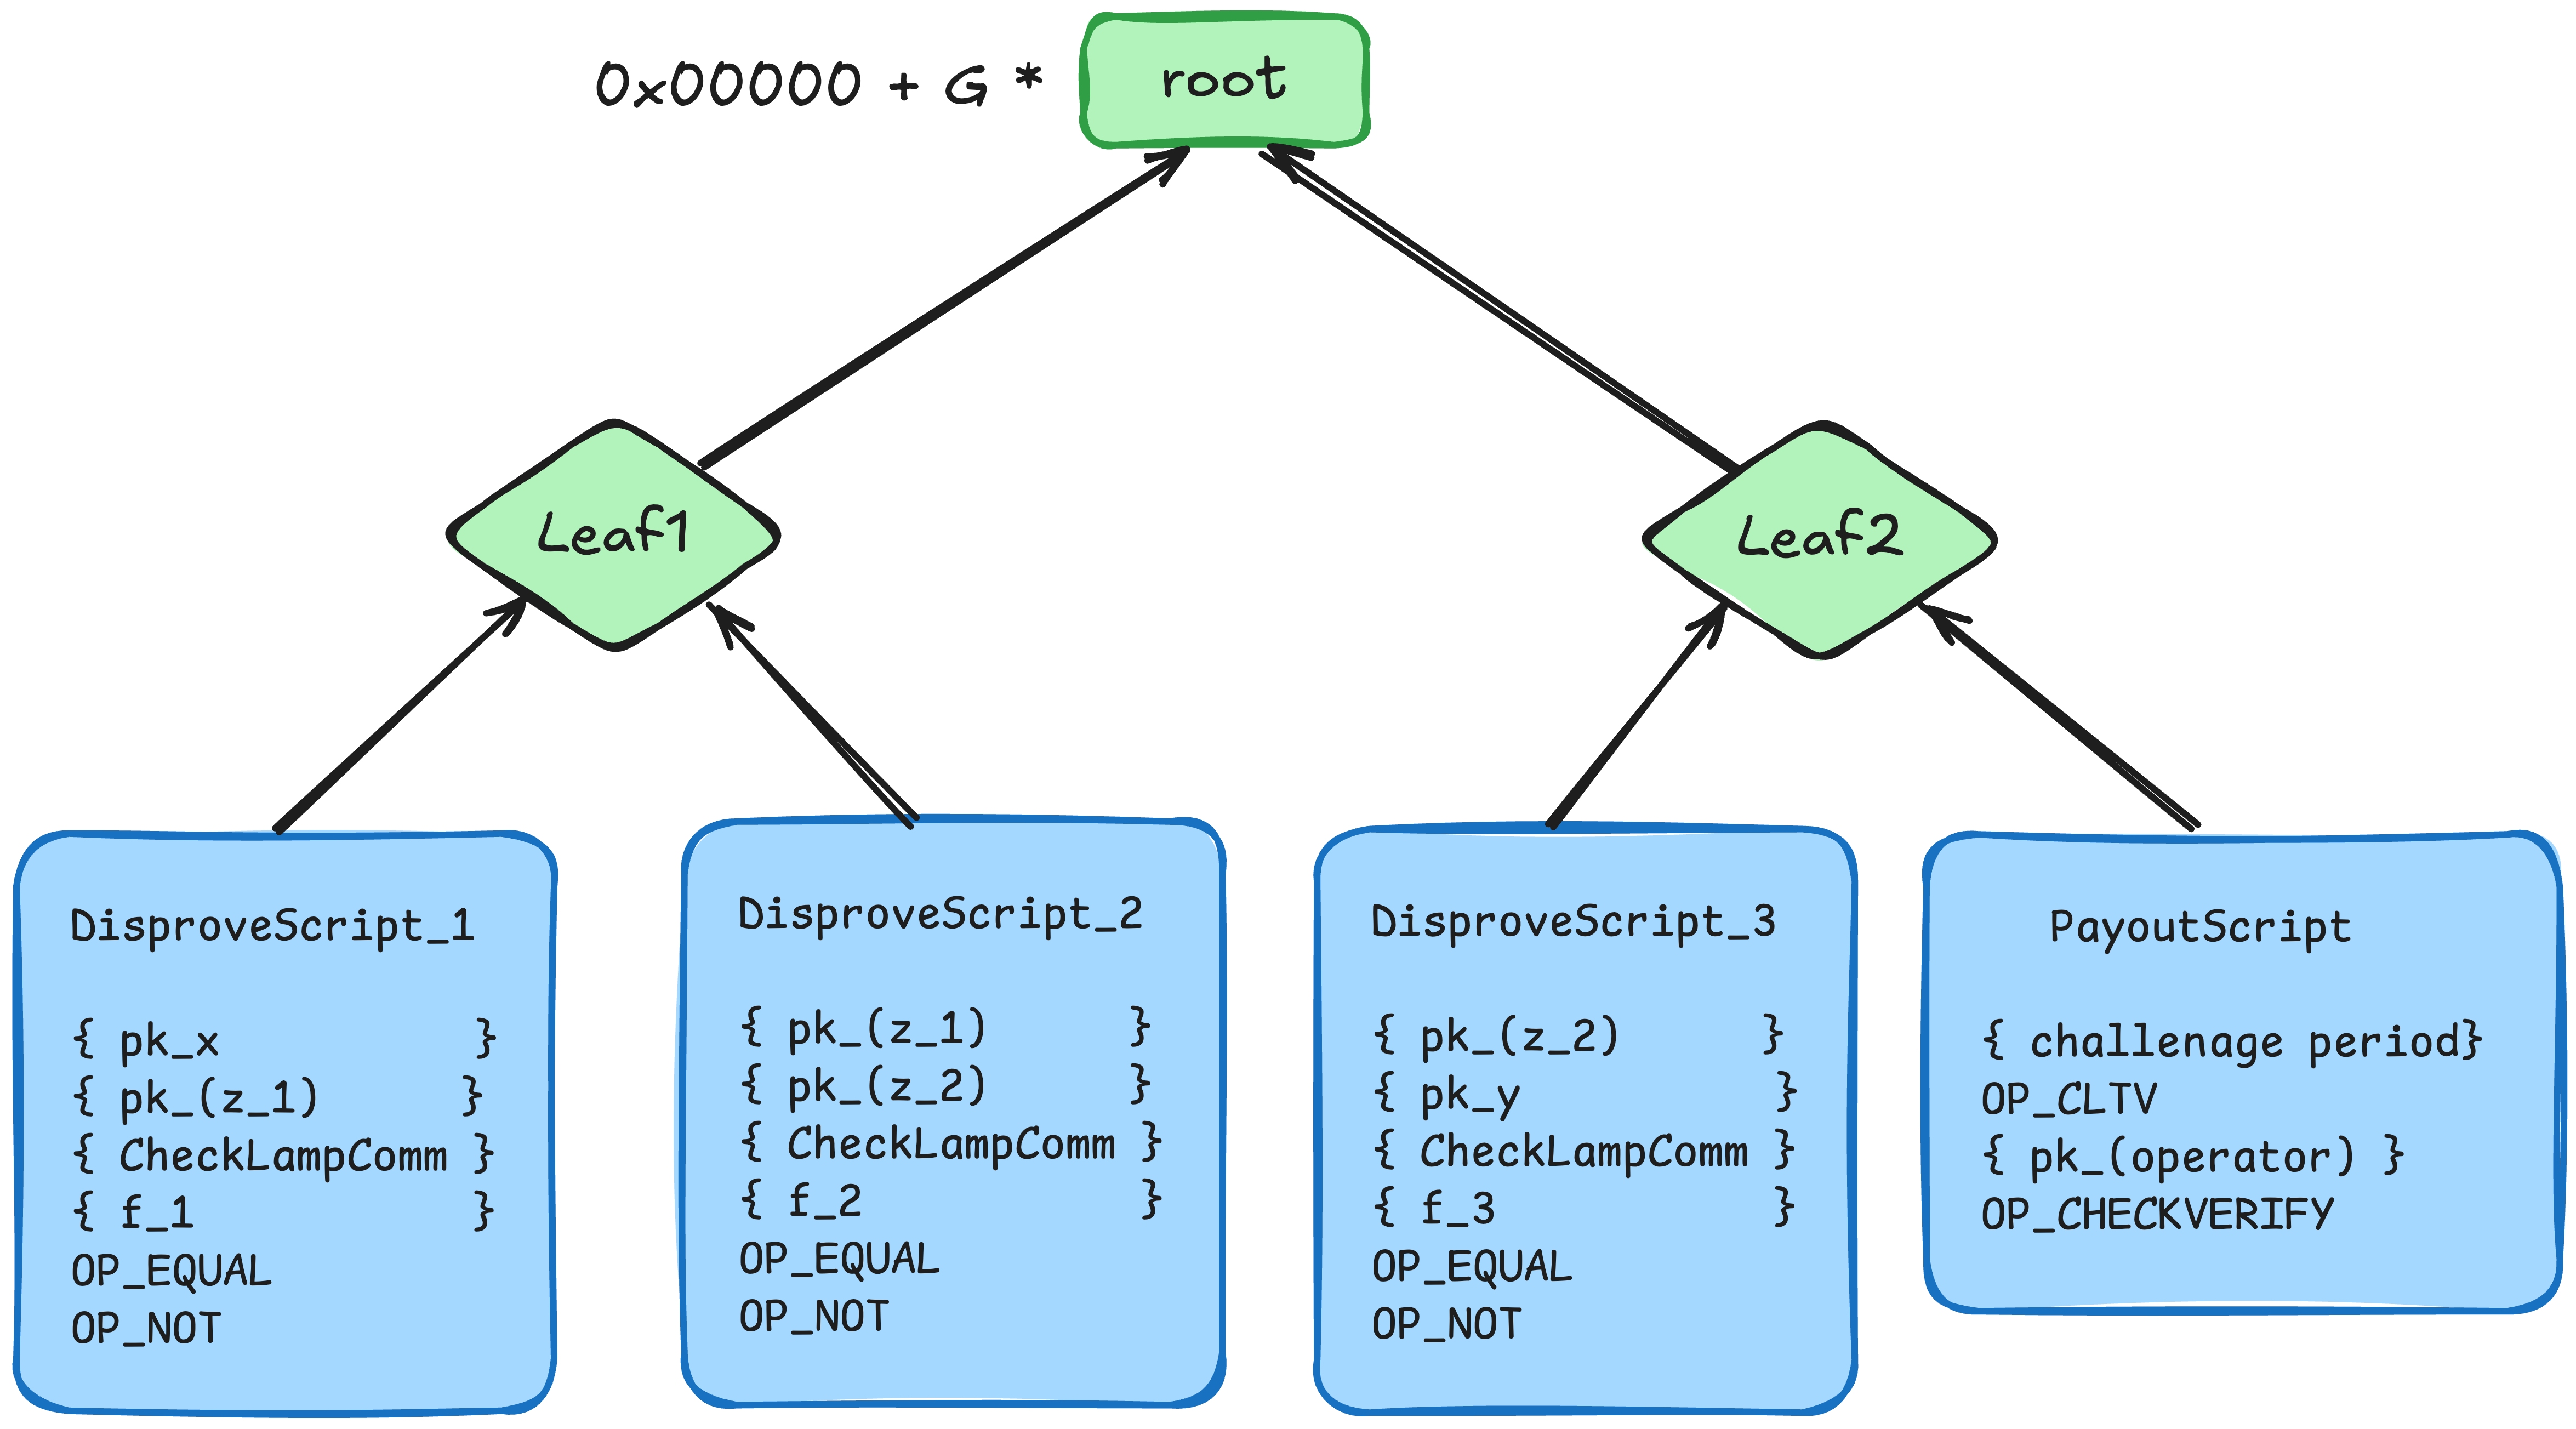
\includegraphics[width=.65\linewidth]{../images/assert-tx-taproot-output.png}
  \caption{\label{fig:assert-tx-mast-tree}Script tree in a Taproot
  address with three sub-programs and two intermediate states.}
\end{figure}


\begin{figure}[htbp]
  \centering
  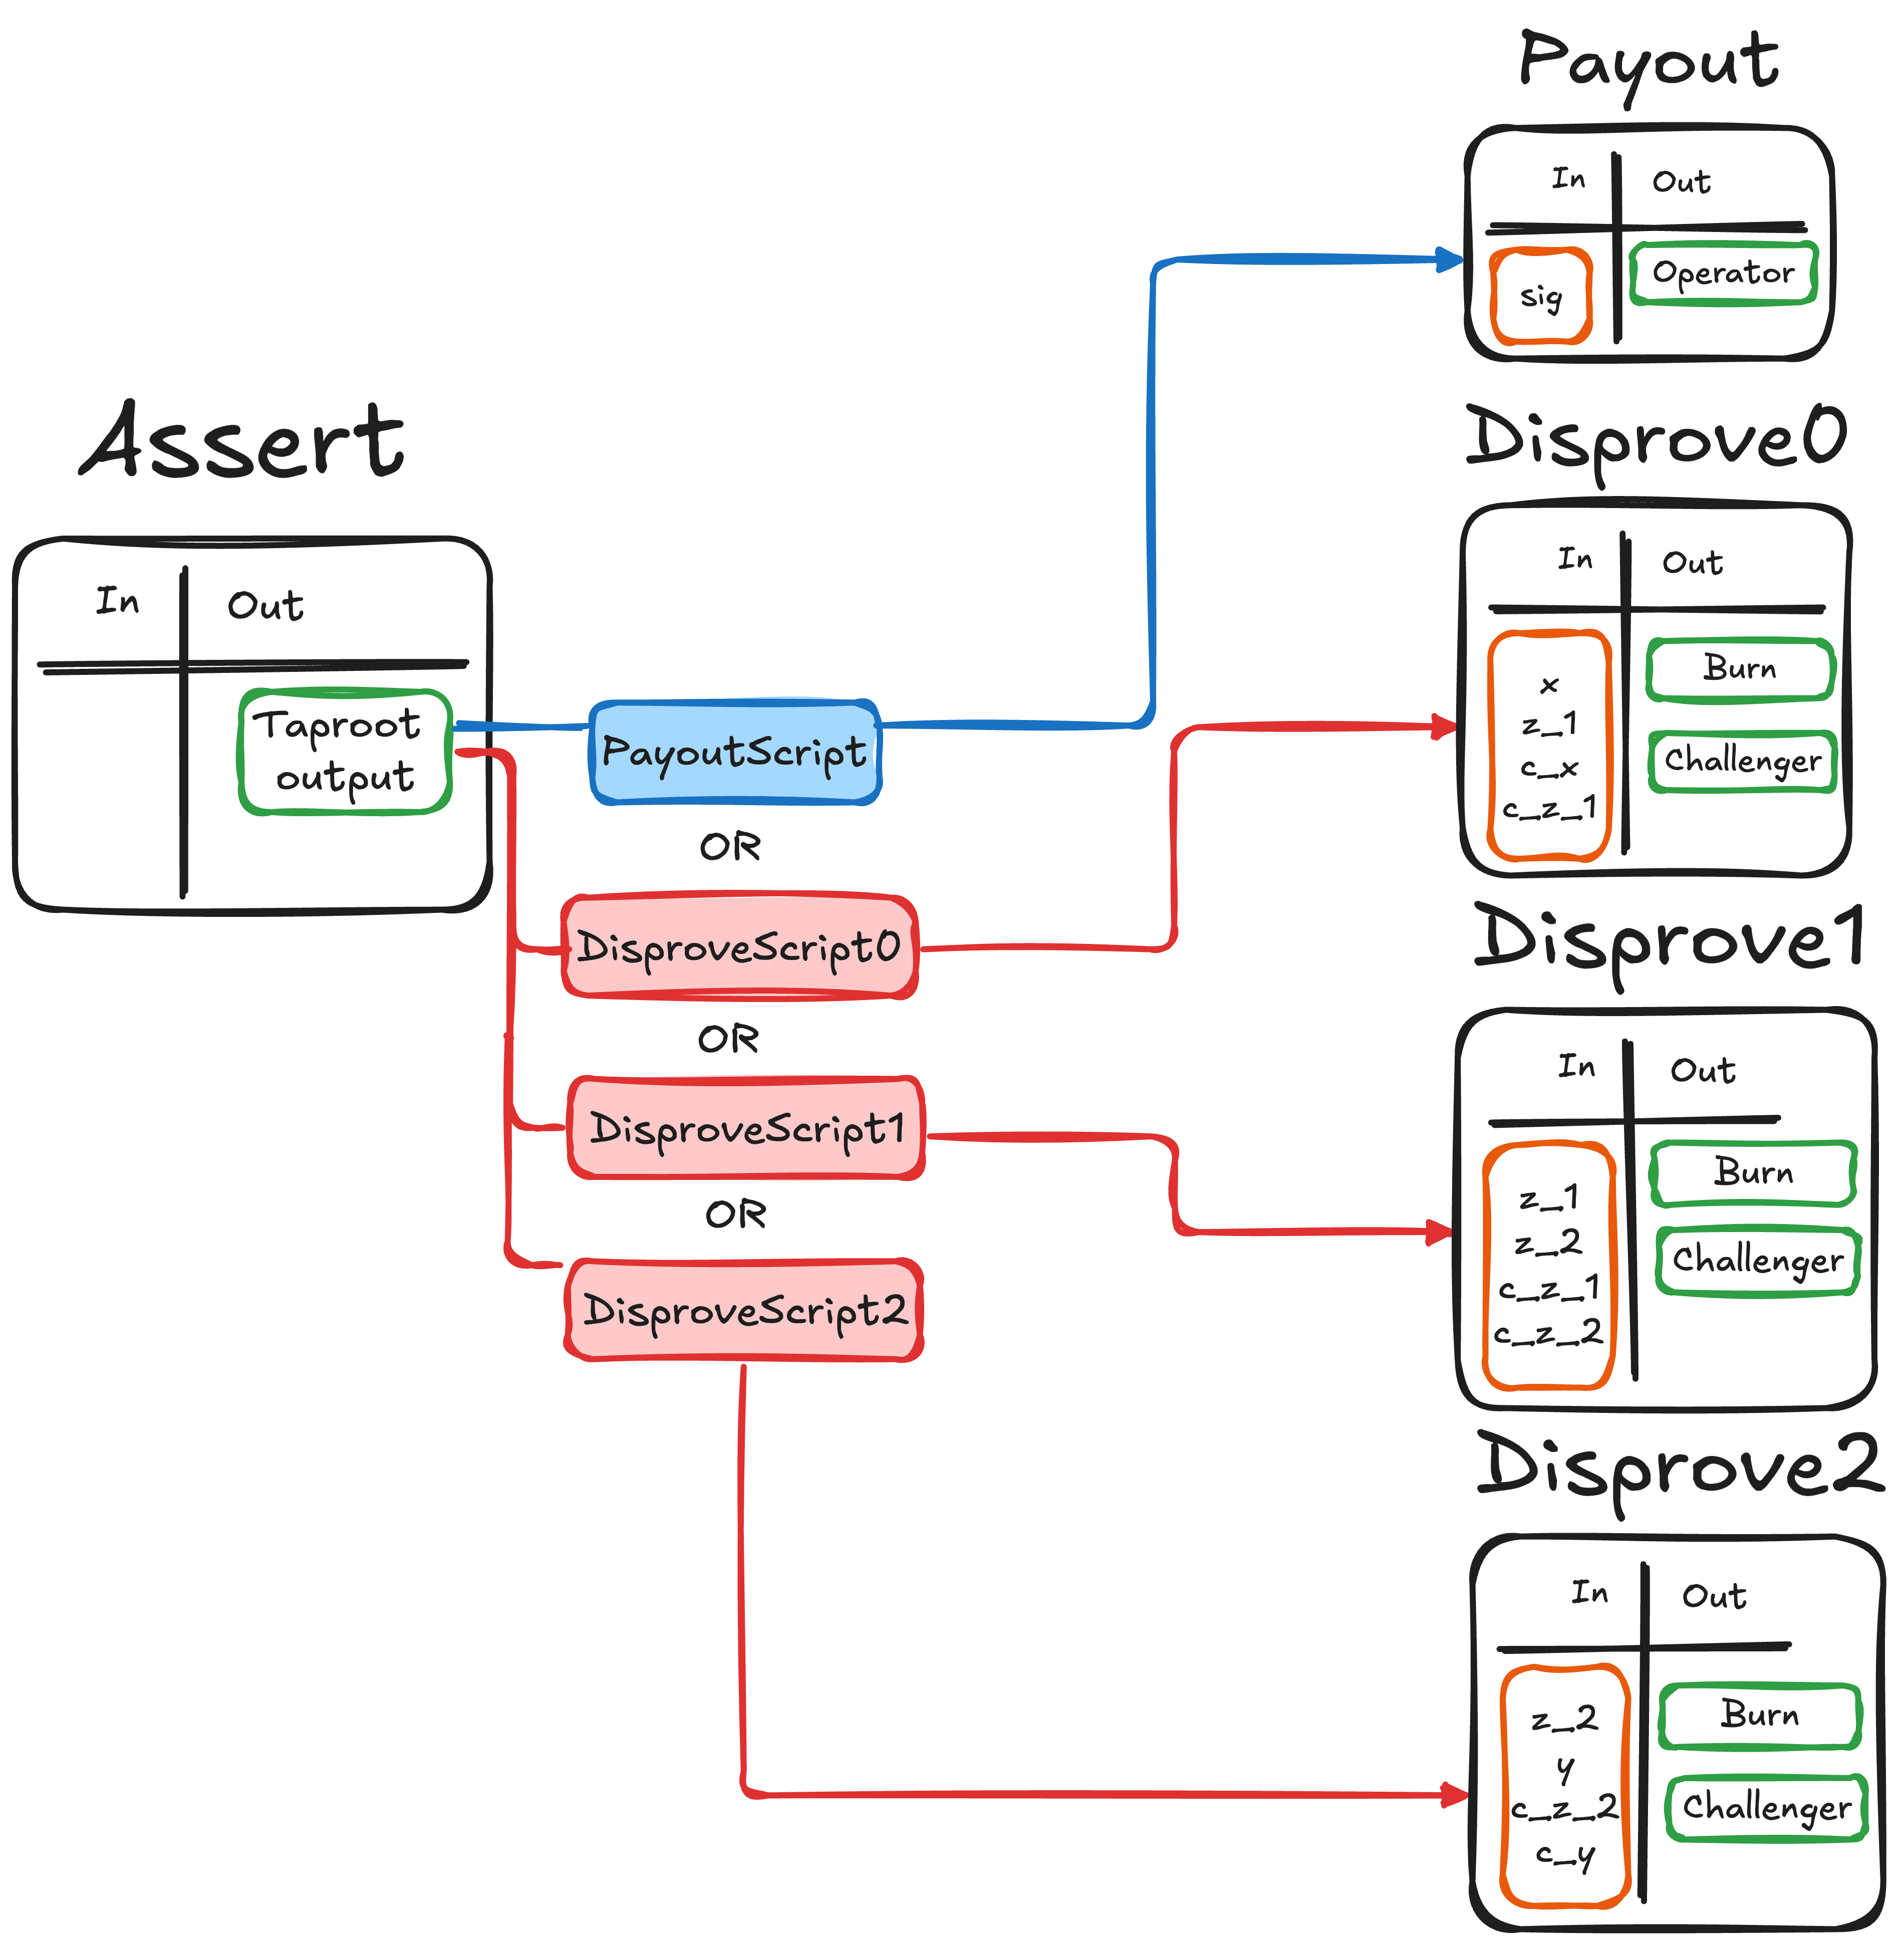
\includegraphics[width=.9\linewidth]{../images/bitvm-txs.png}
  \caption{\label{fig:bitvm-txs}Sequance of transactions in BitVM2
  with 3 subprograms and 2 intermediate states.}
\end{figure}

\pagebreak
\section{Toy Example: Square Fibonacci Sequnce}\label{sec:covenants-emulation}

Let us consider a toy example of the Square Fibonacci Sequence. Suppose our input is a pair of elements $(x_0,x_1)$ from the field $\mathbb{F}_q$. For the sake of convenience, we choose $\mathbb{F}_q$ to be the prime field of BN254 curve, which is frequently used for zk-SNARKs. Then, our program $f_n$ consists in finding the $(n-1)^{\text{th}}$ element in the sequence:
\begin{equation*}
  x_{j+2} = x_{j+1}^2 + x_j^2, \; \text{over $\mathbb{F}_q$.}
\end{equation*}

Such function has a very natural decomposition. Suppose our state is described by the tuple $(x_j,x_{j+1})$. Consider the transition function $\phi: (x_j, x_{j+1}) \mapsto (x_{j+1}, x_j^2 + x_{j+1}^2)$. In this case, our function $f_n$ can be defined as:
\begin{equation*}
  f_n = \phi^{(n)}(x_0,x_1)[1],
\end{equation*}

where the index $(a, b)[1] = b$ means the second element in the tuple.

Suppose that we have $\mathtt{Fq}$ implemented in the Bitcoin script. Then, the state transition function can be implemented as:
\begin{empheqboxed}
  \begin{align*}
    \opcode{\texttt{FQ::DUP}} \, \opcode{\texttt{Fq::SQUARE}} \elem{2} \opcode{\texttt{Fq::OP\_ROLL}} \, \opcode{\texttt{Fq::SQUARE}} \, \opcode{\texttt{Fq::ADD}}
  \end{align*}
\end{empheqboxed}

The size of this transition is roughly \textit{270 kB} and it requires the storage of 18 elements in the stack, costing additional \textit{18 kB}. So the rough size of \texttt{DisproveScript} is \textbf{290 kB}, which is a lot, but still manageable. In turn, consider the function $f_n$, written in Bitcoin script:
\begin{empheqboxed}
  \begin{align*}
    &\textbf{for} \; i \in \{1,\dots,n\} \; \textbf{do} \\
    & \;\;\;\; \opcode{\texttt{FQ::DUP}} \, \opcode{\texttt{Fq::SQUARE}} \elem{2} \opcode{\texttt{Fq::OP\_ROLL}} \, \opcode{\texttt{Fq::SQUARE}} \, \opcode{\texttt{Fq::ADD}} \\
    & \textbf{end} \\
    & \opcode{\texttt{Fq::SWAP}} \; \opcode{\texttt{Fq::OP\_DROP}}
  \end{align*}
\end{empheqboxed}

For $n=128$, the size is roughly \textbf{35 MB}, which, in contrast, is not manageable. However, the decomposition of the function would make roughly $n$ scripts, each of size \textbf{290 kB}. 

\printbibliography{}

\end{document}
